\section{Introducere}

Scopul acestui proiect este acela de a implementa:
\begin{enumerate}
    \item un program care rezolvă diferite lvl pentru jocul AllOut.
    \item un program care încearcă să rezolve puzzle-ul într-un timp cât mai scurt și cu mișcări cât mai puține.
\end{enumerate} 
\newline
\subsection{Ideea jocului}

"AllOut" este un joc de tip puzzle în care jucătorul trebuie să stingă toate luminițele din matrice prin selectarea celulelor în ordine corectă. Scopul este de a stinge toate luminițele în cel mai scurt timp posibil și cu cele mai puține mișcări. Jocul este disponibil pentru mai multe platforme, inclusiv PC, telefoane mobile și tablete.
\newline
\newline
\begin{figure}[h]
    \centering
    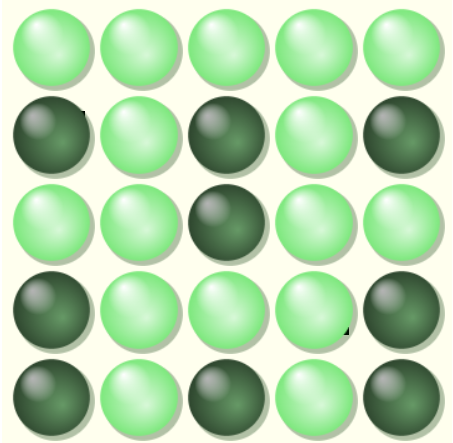
\includegraphics[width=10cm]{text/images/pic1.png}\\
    \caption{Domino}
\end{figure}

Avem nevoie o matrice de n  x n(fiecare n reprezintă un lvl) lumini aprinse sau stinse. Este, de asemenea, nevoie de o strategie și gândire logică pentru a rezolva puzzle-urile mai dificile. Am folosit algortimul de căutare astar.
\newpage

